% Options for packages loaded elsewhere
\PassOptionsToPackage{unicode}{hyperref}
\PassOptionsToPackage{hyphens}{url}
\PassOptionsToPackage{dvipsnames,svgnames,x11names}{xcolor}
%
\documentclass[
  letterpaper,
  DIV=11,
  numbers=noendperiod]{scrartcl}

\usepackage{amsmath,amssymb}
\usepackage{iftex}
\ifPDFTeX
  \usepackage[T1]{fontenc}
  \usepackage[utf8]{inputenc}
  \usepackage{textcomp} % provide euro and other symbols
\else % if luatex or xetex
  \usepackage{unicode-math}
  \defaultfontfeatures{Scale=MatchLowercase}
  \defaultfontfeatures[\rmfamily]{Ligatures=TeX,Scale=1}
\fi
\usepackage{lmodern}
\ifPDFTeX\else  
    % xetex/luatex font selection
\fi
% Use upquote if available, for straight quotes in verbatim environments
\IfFileExists{upquote.sty}{\usepackage{upquote}}{}
\IfFileExists{microtype.sty}{% use microtype if available
  \usepackage[]{microtype}
  \UseMicrotypeSet[protrusion]{basicmath} % disable protrusion for tt fonts
}{}
\makeatletter
\@ifundefined{KOMAClassName}{% if non-KOMA class
  \IfFileExists{parskip.sty}{%
    \usepackage{parskip}
  }{% else
    \setlength{\parindent}{0pt}
    \setlength{\parskip}{6pt plus 2pt minus 1pt}}
}{% if KOMA class
  \KOMAoptions{parskip=half}}
\makeatother
\usepackage{xcolor}
\setlength{\emergencystretch}{3em} % prevent overfull lines
\setcounter{secnumdepth}{-\maxdimen} % remove section numbering
% Make \paragraph and \subparagraph free-standing
\makeatletter
\ifx\paragraph\undefined\else
  \let\oldparagraph\paragraph
  \renewcommand{\paragraph}{
    \@ifstar
      \xxxParagraphStar
      \xxxParagraphNoStar
  }
  \newcommand{\xxxParagraphStar}[1]{\oldparagraph*{#1}\mbox{}}
  \newcommand{\xxxParagraphNoStar}[1]{\oldparagraph{#1}\mbox{}}
\fi
\ifx\subparagraph\undefined\else
  \let\oldsubparagraph\subparagraph
  \renewcommand{\subparagraph}{
    \@ifstar
      \xxxSubParagraphStar
      \xxxSubParagraphNoStar
  }
  \newcommand{\xxxSubParagraphStar}[1]{\oldsubparagraph*{#1}\mbox{}}
  \newcommand{\xxxSubParagraphNoStar}[1]{\oldsubparagraph{#1}\mbox{}}
\fi
\makeatother


\providecommand{\tightlist}{%
  \setlength{\itemsep}{0pt}\setlength{\parskip}{0pt}}\usepackage{longtable,booktabs,array}
\usepackage{calc} % for calculating minipage widths
% Correct order of tables after \paragraph or \subparagraph
\usepackage{etoolbox}
\makeatletter
\patchcmd\longtable{\par}{\if@noskipsec\mbox{}\fi\par}{}{}
\makeatother
% Allow footnotes in longtable head/foot
\IfFileExists{footnotehyper.sty}{\usepackage{footnotehyper}}{\usepackage{footnote}}
\makesavenoteenv{longtable}
\usepackage{graphicx}
\makeatletter
\def\maxwidth{\ifdim\Gin@nat@width>\linewidth\linewidth\else\Gin@nat@width\fi}
\def\maxheight{\ifdim\Gin@nat@height>\textheight\textheight\else\Gin@nat@height\fi}
\makeatother
% Scale images if necessary, so that they will not overflow the page
% margins by default, and it is still possible to overwrite the defaults
% using explicit options in \includegraphics[width, height, ...]{}
\setkeys{Gin}{width=\maxwidth,height=\maxheight,keepaspectratio}
% Set default figure placement to htbp
\makeatletter
\def\fps@figure{htbp}
\makeatother

\usepackage{graphicx}
\DeclareGraphicsExtensions{.pdf,.png,.jpg,.jpeg}
\KOMAoption{captions}{tableheading}
\makeatletter
\@ifpackageloaded{caption}{}{\usepackage{caption}}
\AtBeginDocument{%
\ifdefined\contentsname
  \renewcommand*\contentsname{Table of contents}
\else
  \newcommand\contentsname{Table of contents}
\fi
\ifdefined\listfigurename
  \renewcommand*\listfigurename{List of Figures}
\else
  \newcommand\listfigurename{List of Figures}
\fi
\ifdefined\listtablename
  \renewcommand*\listtablename{List of Tables}
\else
  \newcommand\listtablename{List of Tables}
\fi
\ifdefined\figurename
  \renewcommand*\figurename{Figure}
\else
  \newcommand\figurename{Figure}
\fi
\ifdefined\tablename
  \renewcommand*\tablename{Table}
\else
  \newcommand\tablename{Table}
\fi
}
\@ifpackageloaded{float}{}{\usepackage{float}}
\floatstyle{ruled}
\@ifundefined{c@chapter}{\newfloat{codelisting}{h}{lop}}{\newfloat{codelisting}{h}{lop}[chapter]}
\floatname{codelisting}{Listing}
\newcommand*\listoflistings{\listof{codelisting}{List of Listings}}
\makeatother
\makeatletter
\makeatother
\makeatletter
\@ifpackageloaded{caption}{}{\usepackage{caption}}
\@ifpackageloaded{subcaption}{}{\usepackage{subcaption}}
\makeatother

\ifLuaTeX
  \usepackage{selnolig}  % disable illegal ligatures
\fi
\usepackage{bookmark}

\IfFileExists{xurl.sty}{\usepackage{xurl}}{} % add URL line breaks if available
\urlstyle{same} % disable monospaced font for URLs
\hypersetup{
  pdftitle={Ch3 Lecture 1},
  colorlinks=true,
  linkcolor={blue},
  filecolor={Maroon},
  citecolor={Blue},
  urlcolor={Blue},
  pdfcreator={LaTeX via pandoc}}


\title{Ch3 Lecture 1}
\author{}
\date{}

\begin{document}
\maketitle


\section{\texorpdfstring{\emph{Linear
Independence}}{Linear Independence}}\label{linear-independence}

Why care about linear independence?

\begin{itemize}
\tightlist
\item
  Tells us whether vectors provide ``new information'' or redundantly
  describe the same directions.
\item
  Connects to solving systems: linearly independent columns
  \(\Rightarrow\) at most one solution to \(A\mathbf{x}=\mathbf{b}\).
\end{itemize}

. . .

\subsection{\texorpdfstring{\emph{Linear
Independence}}{Linear Independence}}\label{linear-independence-1}

The vectors \(\mathbf{v}_{1}, \mathbf{v}_{2}, \ldots, \mathbf{v}_{n}\)
are \textbf{linearly dependent} if there exist scalars
\(c_{1}, c_{2}, \ldots, c_{n}\), not all zero, such that

\[
c_{1} \mathbf{v}_{1}+c_{2} \mathbf{v}_{2}+\cdots+c_{n} \mathbf{v}_{n}=\mathbf{0}
\]

Otherwise, the vectors are called \textbf{linearly independent}.

\subsection{\texorpdfstring{\emph{Linear Independence in matrix
form}}{Linear Independence in matrix form}}\label{linear-independence-in-matrix-form}

Let's see if we can rewrite the condition for linear dependence in
matrix form.

\[
c_{1} \mathbf{v}_{1}+c_{2} \mathbf{v}_{2}+\cdots+c_{n} \mathbf{v}_{n}=\mathbf{0}
\]

. . .

Define:

\begin{itemize}
\tightlist
\item
  matrix
  \(A=\left[\mathbf{v}_{1}, \mathbf{v}_{2}, \mathbf{v}_{3}\right]\)
\item
  vector \(\mathbf{c}=\left(c_{1}, c_{2}, c_{3}\right)\).
\end{itemize}

. . .

Then:

\[
c_{1} \mathbf{v}_{1}+c_{2} \mathbf{v}_{2}+c_{3} \mathbf{v}_{3}=\left[\mathbf{v}_{1}, \mathbf{v}_{2}, \mathbf{v}_{3}\right]\left[\begin{array}{l}
c_{1} \\
c_{2} \\
c_{3}
\end{array}\right]=A \mathbf{c}
\]

. . .

Therefore, the vectors
\(\mathbf{v}_1, \mathbf{v}_2, \ldots, \mathbf{v}_n\) are
\textbf{linearly dependent} if there exists a nontrivial (nonzero)
solution to
\([\mathbf{v}_1, \mathbf{v}_2, \ldots, \mathbf{v}_n] \mathbf{c}=\mathbf{0}\).

. . .

Alternatively, we can say that the \emph{columns} of \(A\) are linearly
dependent if there exists a nontrivial solution to
\(A \mathbf{c}=\mathbf{0}\).

\subsection{\texorpdfstring{\emph{The relationship between linear
independence and
invertibility}}{The relationship between linear independence and invertibility}}\label{the-relationship-between-linear-independence-and-invertibility}

The \emph{columns} of \(A\) are \textbf{linearly dependent} if there
exists a nontrivial solution to \(A \mathbf{c}=\mathbf{0}\).

. . .

Conversely, the \emph{columns} of \(A\) are \textbf{linearly
independent} if \(\mathbf{c}=0\) is the only solution to
\(A \mathbf{c}=\mathbf{0}\).

. . .

If the matrix \(A\) happens to be square, we can make a connection to
invertibility.

Remember from the Day 5 lecture, one way of stating that a matrix is
invertible (non-singular) is if \(\mathbf{c}=0\) is the only solution to
\(A \mathbf{c}=\mathbf{0}\).

. . .

Therefore, for an \(n \times n\) matrix \(A\), the columns are
\textbf{linearly independent} if and only if \(A\) is invertible
(non-singular).

\subsection{\texorpdfstring{\emph{Checking for Linear
Independence}}{Checking for Linear Independence}}\label{checking-for-linear-independence}

Is this set of vectors linearly independent?

\[
 \left[\begin{array}{l}1 \\ 1 \\ 0\end{array}\right],\left[\begin{array}{l}0 \\ 1 \\ 1\end{array}\right],\left[\begin{array}{r}1 \\ -1 \\ -2\end{array}\right]
\]

. . .

Goal: find some set of scalars \(c_{1}, c_{2}, c_{3}\), not all zero,
such that
\(c_{1} \mathbf{v}_{1}+c_{2} \mathbf{v}_{2}+c_{3} \mathbf{v}_{3}=\mathbf{0}\).

. . .

How can we do this? We could just guess at some values for
\(c_1, c_2, c_3\) and see if they work\ldots{}

\#\#

Indeed, we can see that \(c_1 = -1, c_2 = 2, c_3 = 1\) works:

\[
\begin{gathered}
-1 \left[\begin{array}{l}1 \\ 1 \\ 0\end{array}\right]
+ 2 \left[\begin{array}{l}0 \\ 1 \\ 1\end{array}\right]
+ 1 \left[\begin{array}{r}1 \\ -1 \\ -2\end{array}\right] \\
=
\left[\begin{array}{l}
-1 \times 1 + 2 \times 0 + 1 \times 1 \\
-1 \times 1 + 2 \times 1 + 1 \times (-1) \\
-1 \times 0 + 2 \times 1 + 1 \times (-2)
\end{array}\right]
=
\left[\begin{array}{l}
-1 + 0 + 1 \\
-1 + 2 - 1 \\
0 + 2 - 2
\end{array}\right]
=
\left[\begin{array}{l}
0 \\
0 \\
0
\end{array}\right]
\end{gathered}
\]

So the vectors are linearly dependent.

. . .

How can we do this more systematically?

\subsection{\texorpdfstring{\emph{Method: Checking for Linear
Independence using Gaussian
Elimination}}{Method: Checking for Linear Independence using Gaussian Elimination}}\label{method-checking-for-linear-independence-using-gaussian-elimination}

\[
 v_1 = \left[\begin{array}{l}1 \\ 1 \\ 0\end{array}\right], v_2 = \left[\begin{array}{l}0 \\ 1 \\ 1\end{array}\right], v_3 = \left[\begin{array}{r}1 \\ -1 \\ -2\end{array}\right]
\]

To check linear independence using Gaussian Elimination, we first need
to construct the matrix \(A\) with the vectors as columns:

\[
A = \left[\mathbf{v}_1\ \mathbf{v}_2\ \mathbf{v}_3\right]
= \left[\begin{array}{rrr}
1 & 0 & 1 \\
1 & 1 & -1 \\
0 & 1 & -2
\end{array}\right]
\]

\subsection{\texorpdfstring{\emph{}}{}}\label{section}

Now we need to find if there is a nontrivial solution to
\(A \mathbf{c}=\mathbf{0}\).

We can build the augmented matrix and find the reduced row echelon form.
Here is the augmented matrix:

\[
\left[\begin{array}{rrr|r}
1 & 0 & 1 & 0 \\
1 & 1 & -1 & 0 \\
0 & 1 & -2 & 0
\end{array}\right]
\]

\subsection{\texorpdfstring{\emph{}}{}}\label{section-1}

\[
\left[\begin{array}{rrr|r}
1 & 0 & 1 & 0 \\
1 & 1 & -1 & 0 \\
0 & 1 & -2 & 0
\end{array}\right]
\]

Our next step is to find the reduced row echelon form of the augmented
matrix.

\[
\left[\begin{array}{rrr|r}
1 & 0 & 1 & 0 \\
1 & 1 & -1 & 0 \\
0 & 1 & -2 & 0
\end{array}\right] \xrightarrow[E_{21}(-1)]{\longrightarrow}\left[\begin{array}{rrr|r}
1 & 0 & 1 & 0 \\
0 & 1 & -2 & 0 \\
0 & 1 & -2 & 0
\end{array}\right] \xrightarrow[E_{32}(-1)]{\longrightarrow}\left[\begin{array}{rrr|r}
1 & 0 & 1 & 0 \\
0 & 1 & -2 & 0 \\
0 & 0 & 0 & 0
\end{array}\right],
\]

\subsection{\texorpdfstring{\emph{Simplification when solving
homogeneous
systems}}{Simplification when solving homogeneous systems}}\label{simplification-when-solving-homogeneous-systems}

Actually, since the last column was all zeros, nothing happened to it
during the row operations.

(Remember, when the right-hand side is all zeros, we call the system
\emph{homogeneous}.)

. . .

It would have been slightly simpler to just leave it off and find the
reduced row echelon form of the matrix \(A\):

. . .

\[
\left[\begin{array}{rrr}
1 & 0 & 1 \\
1 & 1 & -1 \\
0 & 1 & -2
\end{array}\right] \xrightarrow[E_{21}(-1)]{\longrightarrow}\left[\begin{array}{rrr}
1 & 0 & 1 \\
0 & 1 & -2 \\
0 & 1 & -2
\end{array}\right] \xrightarrow[E_{32}(-1)]{\longrightarrow}\left[\begin{array}{rrr}
1 & 0 & 1 \\
0 & 1 & -2 \\
0 & 0 & 0
\end{array}\right],
\]

\subsection{\texorpdfstring{\emph{}}{}}\label{section-2}

Either way, we are left with the following system to solve for
\(\mathbf{c}\):

\[
\left[\begin{array}{rrr}
1 & 0 & 1 \\
0 & 1 & -2 \\
0 & 0 & 0
\end{array}\right]
\left[\begin{array}{c}
c_1 \\ c_2 \\ c_3
\end{array}\right]
=
\left[\begin{array}{c}
0 \\ 0 \\ 0
\end{array}\right]
\]

. . .

This corresponds to the system of equations:

\[
\begin{gathered}
c_1 + c_3 = 0 \\
c_2 - 2c_3 = 0 \\
0 = 0
\end{gathered}
\]

. . .

We see that \(c_3\) is free, and then \(c_1 = -c_3\) and \(c_2 = 2c_3\).

. . .

Setting \(c_3 = 1\), we get \(c_1 = -1\) and \(c_2 = 2\) -- our original
guess!

. . .

But let's not forget to circle back to the original question: because we
found a nontrivial solution to \(A \mathbf{c}=\mathbf{0}\), the vectors
are \textbf{linearly dependent}.

\subsection{\texorpdfstring{\emph{Steps to check for linear independence
using Gaussian
Elimination}}{Steps to check for linear independence using Gaussian Elimination}}\label{steps-to-check-for-linear-independence-using-gaussian-elimination}

\begin{enumerate}
\def\labelenumi{\arabic{enumi}.}
\tightlist
\item
  Set up matrix \(A\) with the vectors as columns.
\item
  Build the augmented matrix \(A | \mathbf{0}\).
\item
  Find the reduced row echelon form of the augmented matrix.
\item
  Check if there is a nontrivial solution to
  \(A \mathbf{c}=\mathbf{0}\).
\end{enumerate}

. . .

If there is a nontrivial solution, the vectors are linearly dependent.
If there is no nontrivial solution, the vectors are linearly
independent.

\subsection{\texorpdfstring{\emph{The relationship between linear
independence and
determinants}}{The relationship between linear independence and determinants}}\label{the-relationship-between-linear-independence-and-determinants}

A few slides back, we saw the columns of a square matrix \(A\) are
independent if and only if \(A\) is invertible.

. . .

Last lecture, we also saw that the determinant of a square matrix \(A\)
is non-zero if and only if \(A\) is invertible.

. . .

Putting these two together, we see that the columns of a square matrix
\(A\) are independent if and only if the determinant of \(A\) is
non-zero.

\subsection{\texorpdfstring{\emph{Method: Checking for Linear
Independence using
Determinants}}{Method: Checking for Linear Independence using Determinants}}\label{method-checking-for-linear-independence-using-determinants}

This leads to our second method for checking for linear independence:

\begin{enumerate}
\def\labelenumi{\arabic{enumi}.}
\tightlist
\item
  Set up matrix \(A\) with the vectors as columns.
\item
  Calculate the determinant of \(A\).
\item
  Check if the determinant is non-zero.
\end{enumerate}

. . .

If the determinant is non-zero, the vectors are linearly independent. If
the determinant is zero, the vectors are linearly dependent.

\subsection{\texorpdfstring{\emph{Example
2}}{Example 2}}\label{example-2}

Are the following vectors linearly independent?

\(\left[\begin{array}{l}0 \\ 1 \\ 0\end{array}\right],\left[\begin{array}{l}1 \\ 1 \\ 0\end{array}\right],\left[\begin{array}{l}0 \\ 1 \\ 1\end{array}\right]\)

. . .

Set up A =
\(\left[\begin{array}{lll}0 & 1 & 0 \\ 1 & 1 & 1 \\ 0 & 0 & 1\end{array}\right]\)

. . .

What is the determinant of \(A\)? Let's work across the top row:

\[
\begin{gather}
\operatorname{det}\left[\begin{array}{lll}
0 & 1 & 0 \\
1 & 1 & 1 \\
0 & 0 & 1
\end{array}\right]
= 0 \times \operatorname{det}\left[\begin{array}{ll}
1 & 1 \\
0 & 1
\end{array}\right]
- 1 \times \operatorname{det}\left[\begin{array}{ll}
1 & 1 \\
0 & 1
\end{array}\right] 
+ 0 \times \operatorname{det}\left[\begin{array}{ll}
1 & 1 \\
0 & 0
\end{array}\right] \\
= -1 \times \operatorname{det}\left[\begin{array}{ll}
1 & 0 \\
0 & 1
\end{array}\right]
= -1
\end{gather}
\]

. . .

Determinant is non-zero, so \(A\) is invertible (non-singular)

. . .

So the vectors are linearly \textbf{independent}.

\subsection{\texorpdfstring{\emph{Comparing the methods: using Gaussian
Elimination to check for linear
independence}}{Comparing the methods: using Gaussian Elimination to check for linear independence}}\label{comparing-the-methods-using-gaussian-elimination-to-check-for-linear-independence}

Let's try our first method with the same example:

\[
A = \left[\begin{array}{ccc}
0 & 1 & 0 \\
1 & 1 & 1 \\
0 & 0 & 1
\end{array}\right]
\]

We want to find if there is a nontrivial solution to
\(A \mathbf{c}=\mathbf{0}\).

. . .

Doing Gaussian Elimination on \(A\), we get: \[
\left[\begin{array}{ccc|c}
0 & 1 & 0 & 0 \\
1 & 1 & 1 & 0 \\
0 & 0 & 1 & 0
\end{array}\right] 
\xrightarrow{E_{12}}
\left[\begin{array}{ccc|c}
1 & 1 & 1 & 0 \\
0 & 1 & 0 & 0 \\
0 & 0 & 1 & 0
\end{array}\right]
\xrightarrow{E_{12}(-1)}
\left[\begin{array}{ccc|c}
1 & 0 & 1 & 0 \\
0 & 1 & 0 & 0 \\
0 & 0 & 1 & 0
\end{array}\right]
\]

\subsection{\texorpdfstring{\emph{}}{}}\label{section-3}

Our RREF is: \[
\left[\begin{array}{ccc|c}
1 & 0 & 1 & 0 \\
0 & 1 & 0 & 0 \\
0 & 0 & 1 & 0
\end{array}\right]
\]

. . .

Then we need to solve

\[
\left[\begin{array}{ccc}
1 & 0 & 1 \\
0 & 1 & 0 \\
0 & 0 & 1
\end{array}\right]
\left[\begin{array}{c}
c_1 \\ c_2 \\ c_3
\end{array}\right]
= \left[\begin{array}{c}
0 \\ 0 \\ 0
\end{array}\right]
\]

This corresponds to the system of equations:

\[
\begin{gather}
c_1 + c_3 = 0 \\
c_2 = 0 \\
c_3 = 0
\end{gather}
\]

. . .

We see that \(c_3\) must be zero, and then \(c_1 = -c_3 = 0\) and
\(c_2 = 0\).

. . .

The only solution is the trivial solution \(\mathbf{c}=0\), so the
vectors are linearly independent.

\subsection{\texorpdfstring{\emph{Summary}}{Summary}}\label{summary}

\begin{itemize}
\tightlist
\item
  The vectors \(v_1, v_2, \ldots, v_n\) are linearly independent if and
  only if the only solution to
  \([\mathbf{v}_1, \mathbf{v}_2, \ldots, \mathbf{v}_n] \mathbf{c}=\mathbf{0}\)
  is \(\mathbf{c}=0\).
\item
  If we define \(A=[\mathbf{v}_1, \mathbf{v}_2, \ldots, \mathbf{v}_n]\),
  the vectors are linearly independent if and only if the only solution
  to \(A \mathbf{c}=0\) is \(\mathbf{c}=0\).
\item
  We can check this by either using Gaussian Elimination or calculating
  the determinant of \(A\).
\end{itemize}

\subsection{\texorpdfstring{\emph{Skills: Linear
Independence}}{Skills: Linear Independence}}\label{skills-linear-independence}

\begin{itemize}
\tightlist
\item
  Describe linear independence in terms of solutions to
  \(v_1 c_1 + v_2 c_2 + \ldots + v_n c_n = \mathbf{0}\).
\item
  Construct a matrix \(A\) with the vectors as columns and use Gaussian
  Elimination or determinants to check for linear independence.
\item
  Interpret linear dependence in terms of solutions to
  \(A\mathbf{c}=\mathbf{0}\).
\end{itemize}

\section{\texorpdfstring{\emph{Vector
Spaces}}{Vector Spaces}}\label{vector-spaces}

We've been working with vectors in \(\mathbb{R}^n\) and linear
combinations. To talk about ``spanning'' and ``bases'' in a precise way,
we need a name for the kind of set we're in: a \textbf{vector space}.

. . .

\subsection{\texorpdfstring{\emph{What is a vector
space?}}{What is a vector space?}}\label{what-is-a-vector-space}

A \textbf{vector space} (over \(\mathbb{R}\)) is a nonempty set \(V\) of
vectors (fixed length \(n\)) together with addition and scalar
multiplication such that:

\begin{itemize}
\tightlist
\item
  \textbf{Closure:} \(\mathbf{u}+\mathbf{v} \in V\) and
  \(c\mathbf{u} \in V\) for all \(\mathbf{u},\mathbf{v} \in V\) and
  scalars \(c\).
\item
  \textbf{Usual rules:} commutativity, associativity, zero, negatives,
  distributivity, and \(1\cdot\mathbf{u}=\mathbf{u}\) (the same rules we
  use in \(\mathbb{R}^n\)).
\end{itemize}

. . .

\subsection{\texorpdfstring{\emph{Examples of vector
spaces}}{Examples of vector spaces}}\label{examples-of-vector-spaces}

\begin{itemize}
\item
  \textbf{\(\mathbb{R}^n\)} --- the set of all \(n\)-tuples with
  standard addition and scalar multiplication. Our main example.
\item
  \textbf{\(\mathbb{R}^2\) and \(\mathbb{R}^3\)} --- the plane and space
  we visualize.
\item
  \textbf{A line through the origin in \(\mathbb{R}^2\)} --- all
  multiples of a fixed nonzero vector:
  \(\{c(x_0,y_0) \mid c \in \mathbb{R}\}\). Adding or scaling vectors in
  this set keeps us in the set, so it is a vector space.
\end{itemize}

. . .

\subsection{\texorpdfstring{\emph{Skills: Vector
Spaces}}{Skills: Vector Spaces}}\label{skills-vector-spaces}

\begin{itemize}
\tightlist
\item
  Say what a vector space is (set of vectors, addition, scalar
  multiplication, closure + usual rules).
\item
  Recognize \(\mathbb{R}^n\), \(\mathbb{R}^2\), \(\mathbb{R}^3\), and
  lines through the origin as vector spaces.
\end{itemize}

\section{\texorpdfstring{\emph{Bases and Spanning
Sets}}{Bases and Spanning Sets}}\label{bases-and-spanning-sets}

\textbf{Why do we care about spanning sets and bases?}

\begin{itemize}
\item
  \textbf{Spanning set:} a set of vectors whose linear combinations give
  us every vector in some collection we care about. Answer to ``can we
  build what we need from these?''
\item
  \textbf{Redundancy:} often one of those vectors is itself a linear
  combination of the others---we are carrying more than we need.
\item
  \textbf{Basis:} a spanning set with no redundancy (linearly
  independent). The most economical way to generate that collection.
\end{itemize}

\subsection{\texorpdfstring{\emph{Basis of a Vector
Space}}{Basis of a Vector Space}}\label{basis-of-a-vector-space}

A \textbf{spanning set} is a set of vectors that can be combined to
create any vector in the vector space.

A \textbf{basis} for the vector space \(V\) is a \emph{spanning} set of
vectors \(\mathbf{v}_{1}, \mathbf{v}_{2}, \ldots, \mathbf{v}_{n}\) that
is a \emph{linearly independent} set.

\subsection{\texorpdfstring{\emph{Standard
Basis}}{Standard Basis}}\label{standard-basis}

The \textbf{standard basis} for \(\mathbb{R}^{n}\) is the set of vectors
\(\mathbf{e}_{1}, \mathbf{e}_{2}, \ldots, \mathbf{e}_{n}\) given by the
columns of the \(n \times n\) identity matrix.

. . .

\subsection{\texorpdfstring{\emph{Showing that the Standard Basis is a
Basis for the reals or complex
numbers}}{Showing that the Standard Basis is a Basis for the reals or complex numbers}}\label{showing-that-the-standard-basis-is-a-basis-for-the-reals-or-complex-numbers}

\begin{itemize}
\tightlist
\item
  Let \(\mathbf{v}=\left(c_{1}, c_{2}, \ldots, c_{n}\right)\) be a
  vector from \(V\)
\item
  \(c_{1}, c_{2}, \ldots, c_{n}\) are scalars (real or complex)
\end{itemize}

. . .

\[
\begin{aligned}
\mathbf{v} & =\left[\begin{array}{c}
c_{1} \\
c_{2} \\
\vdots \\
c_{n}
\end{array}\right]=c_{1}\left[\begin{array}{c}
1 \\
0 \\
\vdots \\
0
\end{array}\right]+c_{2}\left[\begin{array}{c}
0 \\
1 \\
\vdots \\
0
\end{array}\right]+\cdots+c_{n}\left[\begin{array}{c}
0 \\
\vdots \\
0 \\
1
\end{array}\right] \\
& =c_{1} \mathbf{e}_{1}+c_{2} \mathbf{e}_{2}+\cdots+c_{n} \mathbf{e}_{n} .
\end{aligned}
\]

\subsection{\texorpdfstring{\emph{Invertibility, Basis, and Linear
Independence}}{Invertibility, Basis, and Linear Independence}}\label{invertibility-basis-and-linear-independence}

An \(n \times n\) real matrix \(A\) is invertible if and only if its
columns are linearly independent

. . .

in which case they form a basis of \(\mathbb{R}^{n}\)

\subsection{\texorpdfstring{\emph{Skills: Bases and Spanning
Sets}}{Skills: Bases and Spanning Sets}}\label{skills-bases-and-spanning-sets}

You should be able to:

\begin{itemize}
\tightlist
\item
  Identify the standard basis for \(\mathbb{R}^{n}\).
\item
  Explain why a set of vectors forms a basis (spanning + linearly
  independent).
\end{itemize}

\section{\texorpdfstring{\emph{Column Space, Row Space, and Null
Space}}{Column Space, Row Space, and Null Space}}\label{column-space-row-space-and-null-space}

A \textbf{subspace} of \(\mathbb{R}^n\) is a subset that contains
\(\mathbf{0}\) and is closed under addition and scalar multiplication.
Equivalently: \(\mathbf{0} \in W\), and
\(\mathbf{u},\mathbf{v} \in W \Rightarrow \mathbf{u}+\mathbf{v} \in W\),
and
\(\mathbf{u} \in W,\, c \in \mathbb{R} \Rightarrow c\mathbf{u} \in W\).

. . .

Column space, row space, and null space are all subspaces. They
characterize what a matrix ``does.''

\begin{itemize}
\tightlist
\item
  \textbf{Null space} \(\mathcal{N}(A)\): which inputs get mapped to
  \(\mathbf{0}\).
\item
  \textbf{Column space} \(\mathcal{C}(A)\): which outputs are reachable
  as \(A\mathbf{x}\).
\item
  \textbf{Row space} \(\mathcal{R}(A)\): the span of the rows.
\end{itemize}

. . .

\subsection{\texorpdfstring{\emph{Column and Row
Spaces}}{Column and Row Spaces}}\label{column-and-row-spaces}

The \textbf{column space} of the \(m \times n\) matrix \(A\) is the
subspace \(\mathcal{C}(A)\) of \(\mathbb{R}^{m}\) spanned by the columns
of \(A\).

. . .

The \textbf{row space} of the \(m \times n\) matrix \(A\) is the
subspace \(\mathcal{R}(A)\) of \(\mathbb{R}^{n}\) spanned by the
transposes of the rows of \(A\)

\subsection{\texorpdfstring{\emph{Null
Space}}{Null Space}}\label{null-space}

The \textbf{null space} of the \(m \times n\) matrix \(A\) is the subset
\(\mathcal{N}(A)\) of \(\mathbb{R}^{n}\)

\[
\mathcal{N}(A)=\left\{\mathbf{x} \in \mathbb{R}^{n} \mid A \mathbf{x}=\mathbf{0}\right\}
\]

. . .

\(\mathcal{N}(A)\) is just the solution set to
\(A \mathbf{x}=\mathbf{0}\)

. . .

For example, if \(A\) is invertible, \(A \mathbf{x}=\mathbf{0}\) has
only the trivial solution \(\mathbf{x}=\mathbf{0}\)

. . .

so \(\mathcal{N}(A)\) is just \(\left\{\mathbf{0}\right\}\).

. . .

\(A\) is invertible exactly if \(\mathcal{N}(A)=\{\mathbf{0}\}\)

\subsection{\texorpdfstring{\emph{Kernel of an
Operator}}{Kernel of an Operator}}\label{kernel-of-an-operator}

The \textbf{kernel} of the linear operator \(T\) : \(V \rightarrow W\)
is the subspace of \(V\) defined by

\[
\operatorname{ker}(T)=\{\mathbf{x} \in V \mid T(\mathbf{x})=\mathbf{0}\}
\]

For matrix operators kernels are the same thing as null spaces.

\subsection{\texorpdfstring{\emph{Example}}{Example}}\label{example}

Find the null space of the matrix

\[
A=\left[\begin{array}{rrrr}
1 & 1 & 1 & -1 \\
0 & 1 & 2 & 1 
\end{array}\right]
\]

corresponding to the system of equations \[
\begin{aligned}
x_{1}+x_{2}+x_{3}-x_{4} & =0 \\
x_{2}+2 x_{3}+x_{4} & =0
\end{aligned}
\]

. . .

\begin{enumerate}
\def\labelenumi{\arabic{enumi}.}
\tightlist
\item
  Find the RREF of \(A\):
\end{enumerate}

. . .

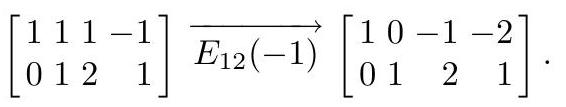
\includegraphics{images/day_8_fig1.jpg}

. . .

\[
\begin{aligned}
& x_{1}=x_{3}+2 x_{4} \\
& x_{2}=-2 x_{3}-x_{4} .
\end{aligned}
\]

\subsection{\texorpdfstring{\emph{}}{}}\label{section-4}

\[
\left[\begin{array}{c}
x_{1} \\
x_{2} \\
x_{3} \\
x_{4}
\end{array}\right]=\left[\begin{array}{c}
x_{3}+2 x_{4} \\
-2 x_{3}-x_{4} \\
x_{3} \\
x_{4}
\end{array}\right]=x_{3}\left[\begin{array}{r}
1 \\
-2 \\
1 \\
0
\end{array}\right]+x_{4}\left[\begin{array}{r}
2 \\
-1 \\
0 \\
1
\end{array}\right] .
\]

. . .

The general solution to the homogeneous system is an arbitrary linear
combination of these two vectors

. . .

\[
\mathcal{N}(A)=\operatorname{span}\left\{\left[\begin{array}{r}
1 \\
-2 \\
1 \\
0
\end{array}\right],\left[\begin{array}{r}
2 \\
-1 \\
0 \\
1
\end{array}\right]\right\} \subseteq \mathbb{R}^{4}
\]

. . .

These are independent, so they form a basis for \(\mathcal{N}(A)\)

\subsection{\texorpdfstring{\emph{Using the Null Space to find a basis
for the column
space}}{Using the Null Space to find a basis for the column space}}\label{using-the-null-space-to-find-a-basis-for-the-column-space}

Find a basis for the column space of the matrix

\[
A=\left[\begin{array}{rrrr}
1 & 1 & 1 & -1 \\
0 & 1 & 2 & 1 
\end{array}\right]
\]

. . .

From before, we found the RREF and used this to find a general form of
the solutions to \(A \mathbf{x}=\mathbf{0}\)

\(\mathbf{x}=\left(x_{1}, x_{2}, x_{3}, x_{4}\right)=\)
\(\left(x_{3}+2 x_{4},-2 x_{3}-x_{4}, x_{3}, x_{4}\right)\)

. . .

Write
\(A=\left[\mathbf{a}_{1}, \mathbf{a}_{2}, \mathbf{a}_{3}, \mathbf{a}_{4}\right]\)

. . .

\(\mathbf{0}=x_{1} \mathbf{a}_{1}+x_{2} \mathbf{a}_{2}+x_{3} \mathbf{a}_{3}+x_{4} \mathbf{a}_{4}\)

. . .

\(\mathbf{0}=\left(x_{3}+2 x_{4}\right) \mathbf{a}_{1}-\left(2 x_{3}+x_{4}\right) \mathbf{a}_{2}+x_{3} \mathbf{a}_{3}+x_{4} \mathbf{a}_{4}\)

. . .

Take \(x_{3}=1\) and \(x_{4}=0\). Then
\(\mathbf{0}=\mathbf{a}_{1}-2 \mathbf{a}_{2}+\mathbf{a}_{3}\)

. . .

So \(\mathbf{a}_{3}\) is a linear combination of \(\mathbf{a}_{1}\) and
\(\mathbf{a}_{2}\)

. . .

Similarly, take \(x_{3}=0\) and \(x_{4}=1\). Then
\(\mathbf{0}=2 \mathbf{a}_{1}-\mathbf{a}_{2}+\mathbf{a}_{4}\) so
\(\mathbf{a}_{4}\) is a linear combination of \(\mathbf{a}_{1}\) and
\(\mathbf{a}_{2}\)

. . .

So \(\mathbf{a}_{1}\) and \(\mathbf{a}_{2}\) are a basis for the column
space of \(A\)

\(\mathcal{C}(A)=\operatorname{span}\left\{\mathbf{a}_{1}, \mathbf{a}_{2}\right\}=\operatorname{span}\left\{\left[\begin{array}{l}1 \\ 0\end{array}\right],\left[\begin{array}{l}1 \\ 1\end{array}\right]\right\}\)

\subsection{\texorpdfstring{\emph{Skills: Fundamental
Subspaces}}{Skills: Fundamental Subspaces}}\label{skills-fundamental-subspaces}

You should be able to:

\begin{itemize}
\tightlist
\item
  Find a basis for the null space of a matrix.
\item
  Find a basis for the column space using the pivot-column / null-space
  method.
\item
  Determine if a matrix is invertible from its null space
  (\(\mathcal{N}(A)=\{\mathbf{0}\}\)).
\end{itemize}

\section{\texorpdfstring{\emph{Applications}}{Applications}}\label{applications}

Applications of null space and column space: finding equilibria,
checking consistency, and describing solution sets.

. . .

\subsection{\texorpdfstring{\emph{Markov chain steady state (finding
equilibrium)}}{Markov chain steady state (finding equilibrium)}}\label{markov-chain-steady-state-finding-equilibrium}

Suppose that a Markov chain has an stable transition matrix
\(A=\left[\begin{array}{ll}0.7 & 0.4 \\ 0.3 & 0.6\end{array}\right]\),
so that

\[
\mathbf{x}^{(k+1)}=A \mathbf{x}^{(k)}
\]

. . .

What is the steady-state vector \(\mathbf{x}\)? (The limit as
\(k \rightarrow \infty\) of \(\mathbf{x}^{(k)}\))

. . .

Take limit of both sides:

\[
\mathbf{x}=A \mathbf{x}
\]

. . .

\[
\mathbf{0}=\mathbf{x}-A \mathbf{x}=I \mathbf{x}-A \mathbf{x}=(I-A) \mathbf{x}
\]

So \(\mathbf{x}\) is in the null space of \(I-A\).

\subsection{\texorpdfstring{\emph{}}{}}\label{section-5}

\[
I-A=\left[\begin{array}{ll}
1 & 0 \\
0 & 1
\end{array}\right]-\left[\begin{array}{ll}
0.7 & 0.4 \\
0.3 & 0.6
\end{array}\right]=\left[\begin{array}{rr}
0.3 & -0.4 \\
-0.3 & 0.4
\end{array}\right] \text {. }
\]

. . .

\[
\left[\begin{array}{rr}
0.3 & -0.4 \\
-0.3 & 0.4
\end{array}\right] \xrightarrow{E_{21}(1)}\left[\begin{array}{rr}
1 & -4 / 3 \\
0 & 0
\end{array}\right]
\]

Solution set is \(x_{1}=4 x_{2} / 3\)

. . .

\[
(3 / 7)(4 / 3,1)=(4 / 7,3 / 7) \approx(0.57143,0.42857)
\]

\subsection{\texorpdfstring{\emph{Consistency and Column Space: Back to
Linear
Systems}}{Consistency and Column Space: Back to Linear Systems}}\label{consistency-and-column-space-back-to-linear-systems}

The linear system \(A \mathbf{x}=\mathbf{b}\) of \(m\) equations in
\(n\) unknowns is consistent if and only if
\(\mathbf{b} \in \mathcal{C}(A)\).

\begin{itemize}
\tightlist
\item
  \(A \mathbf{x}\) is a linear combination of the columns of \(A\) with
  the entries of \(\mathbf{x}\) as scalar coefficients
\item
  If \(A \mathbf{x}=\mathbf{b}\) has a solution means some linear
  combination of columns of \(A\) adds up to \(\mathbf{b}\)
\item
  \(\mathbf{b} \in \mathcal{C}(A)\)
\end{itemize}

\subsection{\texorpdfstring{\emph{How to tell if a vector is in a
spanning
space}}{How to tell if a vector is in a spanning space}}\label{how-to-tell-if-a-vector-is-in-a-spanning-space}

Suppose we have a space \(V\) spanned by
\(\mathbf{v}_{1}=(1,1,3,3), \mathbf{v}_{2}=(0,2,2,4)\), and and
\(\mathbf{v}_{3}=(1,0,2,1)\)

. . .

One of these vectors is in \(V\). Which one?

\(\mathbf{u}=(2,1,5,4)\) and \(\mathbf{w}=(1,0,0,0)\)

. . .

Define \(A=\left[\mathbf{v}_{1}, \mathbf{v}_{2}, \mathbf{v}_{3}\right]\)

Then \(\mathbf{u} \in \mathcal{C}(A)\) if and only if
\(A \mathbf{x}=\mathbf{u}\) has a solution (is consistent)

. . .

Solve both at once: \[
[A|\mathbf{u}| \mathbf{w}]=\left[\begin{array}{lllll}
1 & 0 & 1 & 2 & 1 \\
1 & 2 & 0 & 1 & 0 \\
3 & 2 & 2 & 5 & 0 \\
3 & 4 & 1 & 4 & 0
\end{array}\right] \text { with reduced row echelon form }\left[\begin{array}{rrrrr}
1 & 0 & 1 & 2 & 0 \\
0 & 1 & -\frac{1}{2} & -\frac{1}{2} & 0 \\
0 & 0 & 0 & 0 & 1 \\
0 & 0 & 0 & 0 & 0
\end{array}\right]
\]

. . .

\(\mathbf{u} \in \operatorname{span}\left\{\mathbf{v}_{1}, \mathbf{v}_{2}, \mathbf{v}_{3}\right\}\),

but
\(\mathbf{w} \notin \operatorname{span}\left\{\mathbf{v}_{1}, \mathbf{v}_{2}, \mathbf{v}_{3}\right\}\)

. . .

\[
\mathbf{u}=\left(2-c_{3}\right) \mathbf{v}_{1}+\frac{1}{2}\left(c_{3}-1\right) \mathbf{v}_{2}+c_{3} \mathbf{v}_{3}
\]

\subsection{\texorpdfstring{\emph{Form of general solution to a linear
system}}{Form of general solution to a linear system}}\label{form-of-general-solution-to-a-linear-system}

\begin{itemize}
\item
  Suppose the system \(A \mathbf{x}=\mathbf{b}\) has a particular
  solution \(\mathbf{x}_{*}\).
\item
  Then the general solution \(\mathbf{x}\) to this system can be
  described by the equation
\end{itemize}

\[
\mathbf{x}=\mathbf{x}_{*}+\mathbf{z}
\]

where \(\mathbf{z}\) runs over all elements of \(\mathcal{N}(A)\).

. . .

Solution set is the set of all \textbf{translates} of elements in the
null space of \(A\) by some fixed vector.

. . .

When n is 2 or 3 this says that the solution set is either a single
point, a line or a plane---not necessarily through the origin!

\subsection{\texorpdfstring{\emph{Example}}{Example}}\label{example-1}

Describe the solution sets to the system \[
\begin{array}{r}
x+2 y=3 \\
x+y+t=3 .
\end{array}
\]

. . .

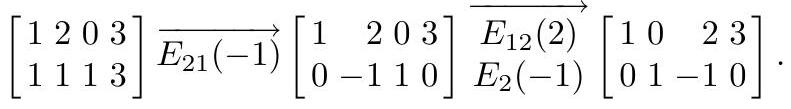
\includegraphics{images/day_8_fig2.jpg}

. . .

\[
\begin{aligned}
& x=3-2 t \\
& y=t \\
& z=t .
\end{aligned}
\]

\subsection{\texorpdfstring{\emph{Gas diffusion in a tube: matrices
simplify physical
systems}}{Gas diffusion in a tube: matrices simplify physical systems}}\label{gas-diffusion-in-a-tube-matrices-simplify-physical-systems}

Diffusion along a line (e.g., gas in a tube) is modeled by a recurrence
like

\[
y_{i, t+1}=y_{i, t}+d\left(y_{i-1, t}-2 y_{i, t}+y_{i+1, t}\right)
\]

with \(d=kD/h^2\). Putting all spatial points into a vector
\(\mathbf{y}_t\), this becomes
\(\mathbf{y}_{t+1}=\mathbf{y}_t+dM\mathbf{y}_t=(I+dM)\mathbf{y}_t\) for
a simple banded matrix \(M\).

. . .

To infer past concentrations from later data we need \(\mathbf{y}_t\)
given \(\mathbf{y}_{t+1}\):

\begin{itemize}
\tightlist
\item
  Exact: \(\mathbf{y}_t=(I+dM)^{-1}\mathbf{y}_{t+1}\) (matrix
  inversion).
\item
  Approximate:
  \(\mathbf{y}_t\approx \mathbf{y}_{t+1}-dM\mathbf{y}_{t+1}\) (replace
  \(\mathbf{y}_t\) by \(\mathbf{y}_{t+1}\) on the right).
\end{itemize}

. . .

Taylor series \((I+dM)^{-1}\approx I-dM+O(d^2)\) shows the two agree to
first order in \(d\). Matrix form made the physics tractable and the
approximation transparent.

\subsection{\texorpdfstring{\emph{Null Space
algorithm}}{Null Space algorithm}}\label{null-space-algorithm}

Given an \(m \times n\) matrix \(A\).

\begin{enumerate}
\def\labelenumi{\arabic{enumi}.}
\item
  Compute the reduced row echelon form \(R\) of \(A\).
\item
  Use \(R\) to find the general solution to the homogeneous system
  \(A \mathbf{x}=0\).
\end{enumerate}

. . .

\begin{enumerate}
\def\labelenumi{\arabic{enumi}.}
\setcounter{enumi}{2}
\tightlist
\item
  Write the general solution
  \(\mathbf{x}=\left(x_{1}, x_{2}, \ldots, x_{n}\right)\) to the
  homogeneous system in the form
\end{enumerate}

\[
\mathbf{x}=x_{i_{1}} \mathbf{w}_{1}+x_{i_{2}} \mathbf{w}_{2}+\cdots+x_{i_{n-r}} \mathbf{w}_{n-r}
\]

where \(x_{i_{1}}, x_{i_{2}}, \ldots, x_{i_{n-r}}\) are the free
variables.

. . .

\begin{enumerate}
\def\labelenumi{\arabic{enumi}.}
\setcounter{enumi}{3}
\tightlist
\item
  List the vectors
  \(\mathbf{w}_{1}, \mathbf{w}_{2}, \ldots, \mathbf{w}_{n-r}\). These
  form a basis of \(\mathcal{N}(A)\).
\end{enumerate}

\subsection{\texorpdfstring{\emph{Skills:
Applications}}{Skills: Applications}}\label{skills-applications}

You should be able to:

\begin{itemize}
\tightlist
\item
  Find steady-state vectors of Markov chains using the null space of
  \(I-A\).
\item
  Determine if \(A\mathbf{x}=\mathbf{b}\) is consistent using column
  space (\(\mathbf{b}\in\mathcal{C}(A)\)).
\item
  Describe solution-set geometry (point, line, plane) using null space
  and particular solutions.
\end{itemize}




\end{document}
